\documentclass[12pt,a4paper]{article}

\usepackage[utf8]{inputenc}
\usepackage[T2A]{fontenc}
\usepackage[ukrainian]{babel}
\usepackage{geometry}
\geometry{
    left=2cm,
    right=2cm,
    top=2cm,
    bottom=2cm
}

\usepackage[table]{xcolor}
\usepackage{amsmath}
\usepackage{graphicx}
\usepackage{subcaption}
\usepackage{multirow}
\usepackage{makecell}
\usepackage{pdflscape}
\usepackage{amsfonts}
\usepackage{array}
\newcolumntype{C}[1]{>{\centering\arraybackslash}m{#1}}

\usepackage[
  unicode,
  pdftitle={ІО-41, Давидчук А.М., Алгоритми та методи обчислень, Лабораторна робота №4},
  pdfauthor={Давидчук Артем},
  pdfsubject={Алгоритми та методи обчислень}
]{hyperref}

\usepackage{minted}

\usemintedstyle{vs}
\setminted{linenos, breaklines, frame=single, fontsize=\small}

\RecustomVerbatimCommand{\VerbatimInput}{VerbatimInput}{
    breaklines=true,
    breaksymbolleft={}
}

\begin{document}

    \begin{titlepage}

        \begin{center}
\includegraphics[width=0.7\textwidth]{../../../TITLES/letterhead.png}\end{center}

        \begin{center}
            \large Національний технічний університет України\\
            «Київський політехнічний інститут імені Ігоря Сікорського»\\[1em]
            Факультет інформатики та обчислювальної техніки\\
            Кафедра обчислювальної техніки
        \end{center}

        \vfill

        \begin{center}
            \textbf{\LARGE Алгоритми та методи обчислень}\\[2em]
            \textbf{\Large Лабораторна робота №4}\\[0.5em]
            «Розв’язання нелінійних рівнянь на комп’ютері»
        \end{center}

        \vfill

        \begin{flushright}
            Виконав: студент 2 курсу ФІОТ, гр. ІО-41\\
            \textit{Давидчук А. М.}\\
            Залікова книжка № 4106\\[1em]
            Перевірив: \textit{Порєв В.\,М.}
        \end{flushright}

        \vfill

        \begin{center}Київ --- 2026\end{center}

    \end{titlepage}

    \noindent
    \textbf{\underline{Тема:}} «Розв’язання нелінійних рівнянь на комп’ютері».

    \vspace{1em}

    \noindent
    \textbf{\underline{Мета:}} Метою даного заняття є ознайомлення з методиками та вивчення різних
алгоритмів розв’язання нелінійних рівнянь на комп’ютері.

    \begin{center} \textbf{\Large Хід роботи} \end{center}

    У даній лабораторній роботі розглядається задача чисельного розв'язання нелінійного рівняння
    методом половинного ділення. Для виконання роботи було обрано рівняння
    \[
        2^x - 4x = 0.
    \]
    Введемо функцію
    \[
        f(x) = 2^x - 4x.
    \]
    Необхідно побудувати графік функції, відокремити корені на заданому проміжку, уточнити їх із
    заданою точністю $\varepsilon$, а також реалізувати програму з графічним інтерфейсом для
    виконання цих дій.

    \vspace{1em}

    \noindent
    \textbf{\underline{Порядок виконання роботи}}:

    \begin{itemize}
        \item Ознайомитись із методикою розв'язання нелінійних рівнянь на ПК.
        \item Побудувати графік функції лівої частини рівняння.
        \item Відокремити корені рівняння на заданому проміжку.
        \item Вибрати значення точності обчислень $\varepsilon$.
        \item На кожному проміжку уточнити корені методом половинного ділення.
        \item Початкові дані та результати обчислень вивести в інтерфейсі програми.
        \item Оформити звіт із описом методу, результатами та програмним кодом.
    \end{itemize}

    \vspace{1em}

    \textbf{\underline{Початкові дані варіанта}}:

    \begin{center}
        \begin{tabular}{|c|c|c|c|}
            \hline
            Рівняння & Метод & Проміжок пошуку & Очікувані корені \\
            \hline
            $2^x - 4x = 0$ & половинного ділення & $[0;4]$ & $0.310;\ 4.0$ \\
            \hline
        \end{tabular}
    \end{center}

    Для тестового запуску програми було використано такі параметри:
    \[
        a = 0,\quad b = 4,\quad h = 0.1,\quad \varepsilon = 10^{-5},\quad N_{\max}=100.
    \]
    Тут $h$ --- крок сканування проміжку для відокремлення коренів, а $N_{\max}$ --- максимальна
    кількість ітерацій уточнення на одному проміжку.

    \vspace{1em}

    \noindent
    \textbf{\underline{Схема алгоритму}}:

    \begin{enumerate}
        \item Задати функцію $f(x)=2^x-4x$, межі $a$, $b$, крок $h$, точність $\varepsilon$ та
        максимальну кількість ітерацій.
        \item Перевірити коректність вхідних даних: $b>a$, $h>0$, $\varepsilon>0$.
        \item Просканувати проміжок $[a;b]$ із кроком $h$.
        \item Для кожної пари сусідніх точок перевірити зміну знака функції.
        \item Сформувати список проміжків, на яких потрібно уточнити корінь.
        \item Для кожного проміжку виконати метод половинного ділення.
        \item На кожній ітерації обчислити середину проміжку та значення функції в ній.
        \item Замінити одну з меж проміжку так, щоб корінь залишився всередині нового проміжку.
        \item Завершити уточнення, коли досягнуто точності $\varepsilon$.
        \item Вивести таблицю результатів, побудувати графік та сформувати текстовий звіт.
    \end{enumerate}

    \vspace{1em}

    \textbf{\underline{Результати обчислень}}:

    Для першого кореня, відокремленого на проміжку $[0.3;0.4]$, отримано таку ітераційну таблицю.

    \begin{center}
        \scriptsize
        \begin{tabular}{|c|c|c|c|c|c|}
            \hline
            $k$ & $a_k$ & $b_k$ & $c_k$ & $f(c_k)$ & $\Delta_k$ \\
            \hline
            1 & 0.3000000000 & 0.4000000000 & 0.3500000000 & $-1.254394\cdot10^{-1}$ & $5.000000\cdot10^{-2}$ \\
            2 & 0.3000000000 & 0.3500000000 & 0.3250000000 & $-4.733556\cdot10^{-2}$ & $2.500000\cdot10^{-2}$ \\
            3 & 0.3000000000 & 0.3250000000 & 0.3125000000 & $-8.142188\cdot10^{-3}$ & $1.250000\cdot10^{-2}$ \\
            4 & 0.3000000000 & 0.3125000000 & 0.3062500000 & $1.148951\cdot10^{-2}$ & $6.250000\cdot10^{-3}$ \\
            5 & 0.3062500000 & 0.3125000000 & 0.3093750000 & $1.670754\cdot10^{-3}$ & $3.125000\cdot10^{-3}$ \\
            6 & 0.3093750000 & 0.3125000000 & 0.3109375000 & $-3.236445\cdot10^{-3}$ & $1.562500\cdot10^{-3}$ \\
            7 & 0.3093750000 & 0.3109375000 & 0.3101562500 & $-7.830272\cdot10^{-4}$ & $7.812500\cdot10^{-4}$ \\
            8 & 0.3093750000 & 0.3101562500 & 0.3097656250 & $4.438179\cdot10^{-4}$ & $3.906250\cdot10^{-4}$ \\
            9 & 0.3097656250 & 0.3101562500 & 0.3099609375 & $-1.696160\cdot10^{-4}$ & $1.953125\cdot10^{-4}$ \\
            10 & 0.3097656250 & 0.3099609375 & 0.3098632813 & $1.370981\cdot10^{-4}$ & $9.765625\cdot10^{-5}$ \\
            11 & 0.3098632813 & 0.3099609375 & 0.3099121094 & $-1.625967\cdot10^{-5}$ & $4.882813\cdot10^{-5}$ \\
            12 & 0.3098632813 & 0.3099121094 & 0.3098876953 & $6.041904\cdot10^{-5}$ & $2.441406\cdot10^{-5}$ \\
            13 & 0.3098876953 & 0.3099121094 & 0.3098999023 & $2.207964\cdot10^{-5}$ & $1.220703\cdot10^{-5}$ \\
            14 & 0.3098999023 & 0.3099121094 & 0.3099060059 & $2.909977\cdot10^{-6}$ & $6.103516\cdot10^{-6}$ \\
            \hline
        \end{tabular}
    \end{center}

    Оскільки на 14-й ітерації виконано умову
    \[
        |f(c_{14})| = 2.909977\cdot10^{-6} \leq 10^{-5},
    \]
    уточнення першого кореня завершується. Другий корінь дорівнює $4.0000000000$, оскільки
    \[
        f(4)=2^4-4\cdot4=16-16=0.
    \]

    Підсумкова таблиця результатів:

    \begin{center}
        \begin{tabular}{|c|c|c|c|c|}
            \hline
            № & Проміжок & Корінь & $f(x)$ & Кількість ітерацій \\
            \hline
            1 & $[0.3000000000;\ 0.4000000000]$ & 0.3099060059 & $2.909977\cdot10^{-6}$ & 14 \\
            \hline
            2 & $x=4.0000000000$ & 4.0000000000 & $0$ & 0 \\
            \hline
        \end{tabular}
    \end{center}

    \newpage

    \noindent
    Блок-схема алгоритму:

    \begin{figure}[h!]
        \centering
        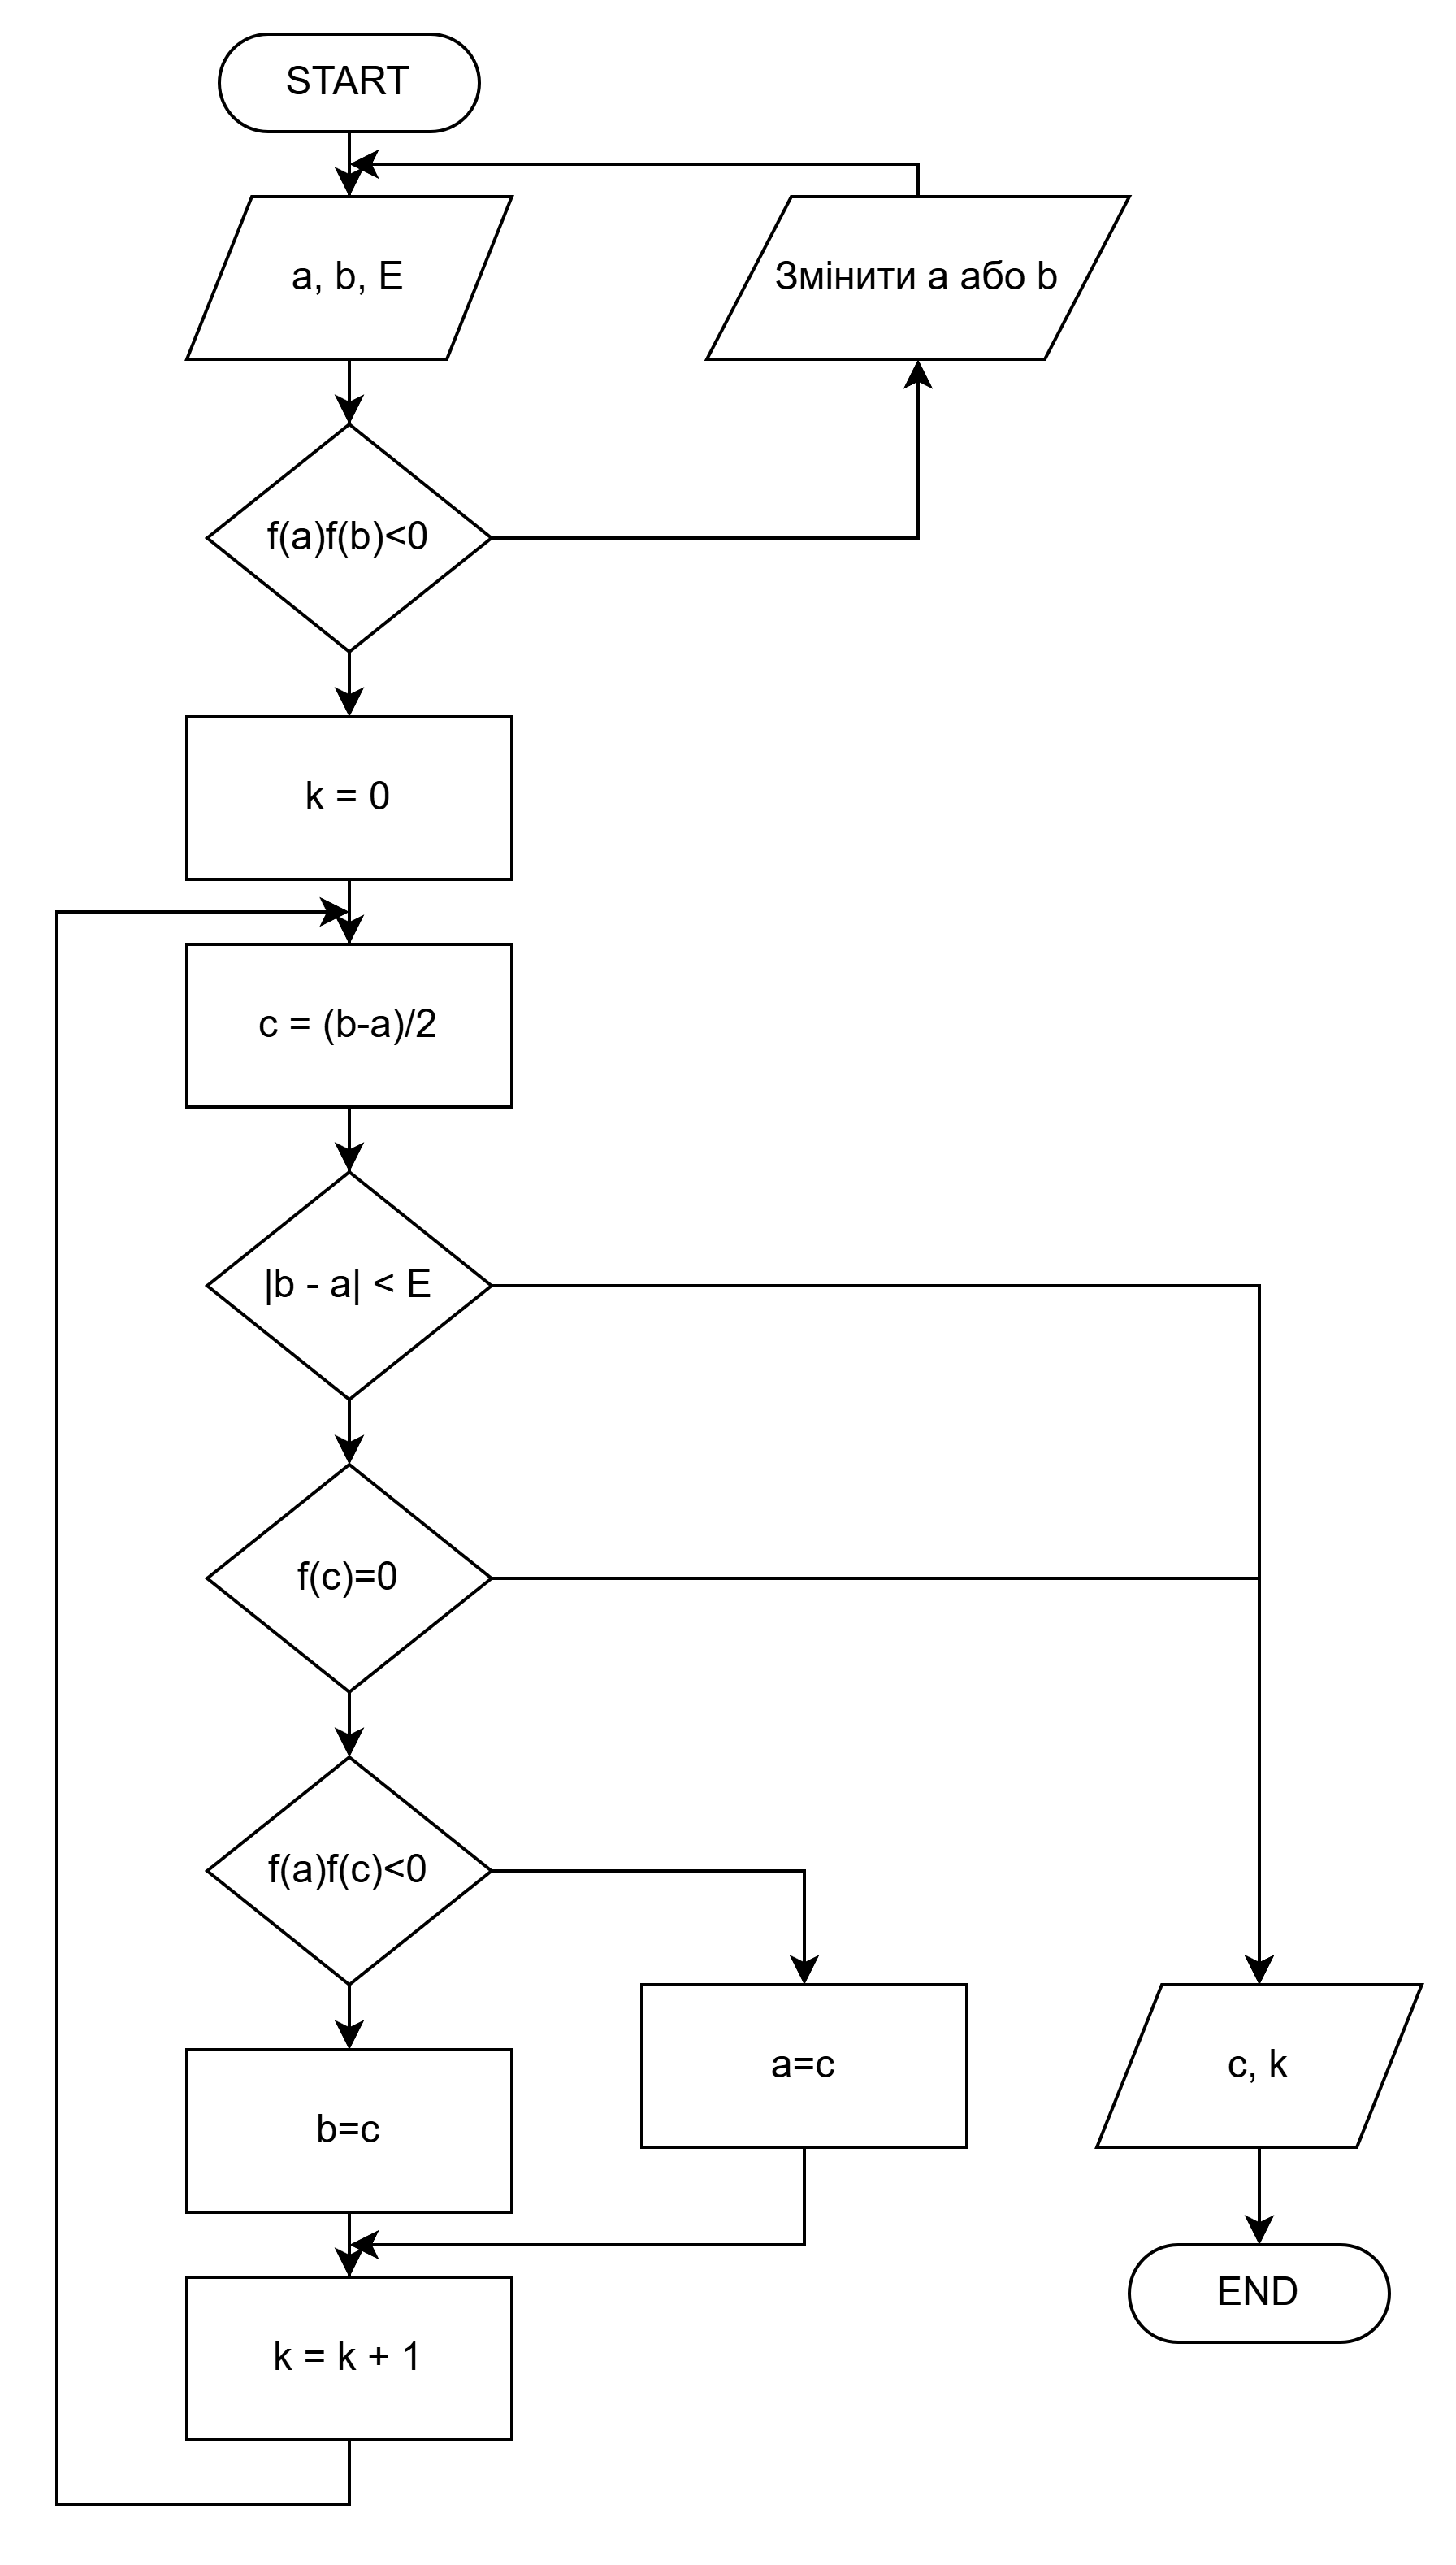
\includegraphics[width=0.7\linewidth]{media/alg.png}
        \caption{Блок-схема алгоритму методу половинного ділення}
    \end{figure}

    \newpage

    \noindent
    \textbf{\underline{Опис програмної реалізації}}:

    \vspace{1em}

    Програма написана мовою Python із розділенням відповідальностей між модулями. Такий підхід
    відповідає базовим інженерним принципам SWEBOK: модульність, зрозумілі межі відповідальності,
    перевірка вхідних даних, відокремлення алгоритмічної частини від графічного інтерфейсу.

    \noindent
    Фактична структура проєкту:

    \begin{verbatim}
project/
|-- app.py
|-- src/
|   |-- bisection.py
|   |-- error_analysis.py
|   |-- functions.py
|   |-- graph_build.py
|   |-- gui.py
|   |-- io_utils.py
|   |-- models.py
|   |-- report.py
|   |-- theme.py
|-- test_json/
    |-- default.json
    |-- high_precision.json
    |-- wide_interval.json
    \end{verbatim}

    \texttt{app.py} відповідає за запуск програми. Модуль \texttt{functions.py} містить цільову
    функцію. Модуль \texttt{bisection.py} реалізує відокремлення коренів та метод половинного
    ділення. Модулі \texttt{models.py}, \texttt{error\_analysis.py}, \texttt{report.py} та
    \texttt{io\_utils.py} відповідають за структури даних, підготовку таблиць, формування звіту та
    роботу з JSON-файлами. Модуль \texttt{graph\_build.py} готує дані для побудови графіка, а
    \texttt{gui.py} реалізує графічний інтерфейс користувача.

    У графічному інтерфейсі передбачено:
    \begin{itemize}
        \item введення меж проміжку, кроку, точності та кількості точок графіка;
        \item завантаження параметрів із JSON-файлу;
        \item запуск обчислень;
        \item виведення таблиці коренів;
        \item збереження текстового звіту;
        \item побудову інтерактивного графіка з можливістю перетягування та масштабування.
    \end{itemize}

    \noindent
    \textbf{\underline{Програмний код}}:

    \vspace{1em}

    \noindent
    \underline{(\texttt{project/app.py})}
    \inputminted{python}{project/app.py}

    \vspace{1em}

    \noindent
    \underline{(\texttt{project/src/models.py})}
    \inputminted{python}{project/src/models.py}

    \vspace{1em}

    \noindent
    \underline{(\texttt{project/src/functions.py})}
    \inputminted{python}{project/src/functions.py}

    \vspace{1em}

    \noindent
    \underline{(\texttt{project/src/bisection.py})}
    \inputminted{python}{project/src/bisection.py}

    \vspace{1em}

    \noindent
    \underline{(\texttt{project/src/error\_analysis.py})}
    \inputminted{python}{project/src/error_analysis.py}

    \vspace{1em}

    \noindent
    \underline{(\texttt{project/src/graph\_build.py})}
    \inputminted{python}{project/src/graph_build.py}

    \vspace{1em}

    \noindent
    \underline{(\texttt{project/src/io\_utils.py})}
    \inputminted{python}{project/src/io_utils.py}

    \vspace{1em}

    \noindent
    \underline{(\texttt{project/src/report.py})}
    \inputminted{python}{project/src/report.py}

    \vspace{1em}

    \noindent
    \underline{(\texttt{project/src/theme.py})}
    \inputminted{python}{project/src/theme.py}

    \vspace{1em}

    \noindent
    \underline{(\texttt{project/src/gui.py})}
    \inputminted{python}{project/src/gui.py}

    \noindent
    \textbf{\underline{Тестові JSON-файли}}:

    Для перевірки завантаження конфігурації було підготовлено три JSON-файли. Стандартний файл
    має такий вигляд:

    \noindent
    \underline{(\texttt{project/test\_json/default.json})}
    \inputminted{json}{project/test_json/default.json}

    Файл із вищою точністю:

    \noindent
    \underline{(\texttt{project/test\_json/high\_precision.json})}
    \inputminted{json}{project/test_json/high_precision.json}

    Файл із ширшим проміжком пошуку:

    \noindent
    \underline{(\texttt{project/test\_json/wide\_interval.json})}
    \inputminted{json}{project/test_json/wide_interval.json}

    \newpage

    \noindent
    \underline{\textbf{Скріншоти демонстрації програми:}}

    \begin{figure}[htbp]
        \centering

        \begin{subfigure}{0.42\textwidth}
            \centering
            
\includegraphics[width=\linewidth]{media/demo1.png}
        \end{subfigure}
        \begin{subfigure}{0.42\textwidth}
            \centering
            
\includegraphics[width=\linewidth]{media/demo2.png}
        \end{subfigure}

        \vspace{1mm}

        \begin{subfigure}{0.42\textwidth}
            \centering
            
\includegraphics[width=\linewidth]{media/demo3.png}
        \end{subfigure}
        \begin{subfigure}{0.42\textwidth}
            \centering
            
\includegraphics[width=\linewidth]{media/demo4.png}
        \end{subfigure}

        \caption{Скріншоти демонстрації програми}

    \end{figure}

    \begin{center} \textbf{\Large Аналіз результатів} \end{center}

    У ході виконання лабораторної роботи було реалізовано програму для розв'язання нелінійного
    рівняння
    \[
        2^x - 4x = 0
    \]
    методом половинного ділення. Спочатку було побудовано логіку відокремлення коренів шляхом
    сканування проміжку з фіксованим кроком. Після цього для кожного знайденого проміжку було
    застосовано метод половинного ділення, який послідовно звужує проміжок локалізації кореня.

    Отримані результати показали, що рівняння має два корені на проміжку $[0;4]$:
    \[
        x_1 \approx 0.3099060059,\quad x_2 = 4.0000000000.
    \]
    Для першого кореня було виконано 14 ітерацій, а значення нев'язки становить
    $2.909977\cdot10^{-6}$, що не перевищує заданої точності $10^{-5}$. Другий корінь є точним,
    оскільки він збігається з правою межею проміжку і дає значення функції $f(4)=0$.

    Розроблена програма дозволяє вводити початкові дані вручну або завантажувати їх із JSON-файлу,
    переглядати результати у таблиці, зберігати звіт та аналізувати функцію за допомогою
    інтерактивного графіка. Це підтверджує коректність реалізації алгоритму та практичну
    придатність програми для дослідження нелінійних рівнянь.


\end{document}
